\documentclass[11pt]{article}

\usepackage{deauthor,times,graphicx}

% JobGraph fig
\usepackage{tikz}
\usetikzlibrary{arrows,automata,positioning,shapes.geometric}

% trademark symbol
\usepackage{textcomp}

\usepackage{float}

% code listings
\usepackage{listings}

\graphicspath{{figs/}}

\newcommand{\TODO}[1]{\textcolor{red}{TODO: #1}}
\newcommand{\sectionautorefname}{Section}%
\newcommand{\para}[1]{\vspace{2mm}\noindent\textbf{#1}}

\definecolor{dkgreen}{rgb}{0,0.6,0}
\definecolor{gray}{rgb}{0.5,0.5,0.5}
\definecolor{mauve}{rgb}{0.58,0,0.82}

% there is no built in support or Scala yet, good enough
\lstset{frame=l,
  language=Java,
  aboveskip=3mm,
  belowskip=3mm,
  showstringspaces=false,
  xleftmargin=5pt,
%   framexleftmargin=-1pt,
  columns=flexible,
  basicstyle={\scriptsize\ttfamily},
  numbers=none,
  numberstyle=\tiny\color{black},
  keywordstyle=\color{blue},
  commentstyle=\color{dkgreen},
  stringstyle=\color{mauve},
  breaklines=true,
  breakatwhitespace=true,
  tabsize=4,
  %for scala
  emph={%  
    object, def, val, zip, window, trigger, evict%
    },emphstyle={\color{blue}\textbf}%
}%


% \usepackage[
% % backend=biber
% % style=alphabetic,
% % sorting=abbrv
% ]{biblatex}

% \renewbibmacro{in:}{}

 
% \addbibresource{references.bib}
% \renewcommand{\bibfont}{\small} % or any other  appropriate font command

% url references
\usepackage[hidelinks]{hyperref}

% in paragraph enums
\usepackage{paralist}

\usepackage{subfig}

\def\definitionautorefname{Definition}
\def\sectionautorefname{Section}
\def\subsectionautorefname{Section}
\def\subsubsectionautorefname{Section}
\def\algorithmautorefname{Algorithm}
\def\figureautorefname{Figure}

\begin{document}

\title{Apache Flink\texttrademark: Stream and Batch Processing in a Single Engine}

\author{Paris Carbone\textsuperscript{$\dagger$} \\ Asterios Katsifodimos\textsuperscript{*} \\\\ \small{ \textsf{\small \textsuperscript{$\dagger$}KTH \& SICS Sweden}} \\ \small \href{parisc,haridi@kth.se}{parisc,haridi@kth.se}
\and Stephan Ewen\textsuperscript{$\ddagger$} \\ Volker Markl\textsuperscript{*} \\\\ \small \textsf{\textsuperscript{$\ddagger$}data Artisans} \\ \small \href{first@data-artisans.com}{first@data-artisans.com}
\and Seif Haridi\textsuperscript{$\dagger$} \\ Kostas Tzoumas\textsuperscript{$\ddagger$} \\\\ \small \textsf{\textsuperscript{*}TU Berlin \& DFKI} \\ \small \href{fist.last@tu-berlin.de}{first.last@tu-berlin.de}
%
\vspace{-5mm}
}

%\and Stefan Ewen$^2$ \and Seif Haridi$^1$ \and Asterios Katsifodimos$^3$ \and Volker Markl$^3$ \and Kostas Tzoumas$^2$}

\maketitle

\begin{abstract}
Apache Flink\footnote{The authors of this paper make no claim in being the sole inventors or implementers of the ideas behind Apache Flink, but rather a group of people that attempt to accurately document Flink's concepts and their significance. Consult \autoref{sec:acknowledgements} for acknowledgements.} is an open-source system for processing streaming and batch data. Flink is built on the philosophy that many classes of data processing applications, including real-time analytics, continuous data pipelines, historic data processing (batch), and iterative algorithms (machine learning, graph analysis) can be expressed and executed as pipelined fault-tolerant dataflows. In this paper, we present Flink's architecture and expand on how a (seemingly diverse) set of use cases can be unified under a single execution model.
\end{abstract}

%!TEX root = paper.tex


\section{Introduction}
\label{sec:intro}
\vspace{-3mm}
Data-stream processing (e.g., as exemplified by complex event processing systems) and static (batch) data processing (e.g., as exemplified by MPP databases and Hadoop) were traditionally considered as two very different types of applications. They were programmed using different programming models and APIs, and were executed by different systems (e.g., dedicated streaming systems such as  Apache Storm, IBM Infosphere Streams, Microsoft StreamInsight, or Streambase versus relational databases or execution engines for Hadoop, including Apache Spark and Apache Drill). Traditionally, batch data analysis made up for the lion's share of the use cases, data sizes, and market, while streaming data analysis mostly served specialized applications.

It is becoming more and more apparent, however, that a huge number of today's large-scale data processing use cases handle data that is, in reality, produced continuously over time. These continuous streams of data come for example from web logs, application logs, sensors, or as changes to application state in databases (transaction log records). Rather than treating the streams as streams, today's setups ignore the continuous and timely nature of data production. Instead, data records are (often artificially) batched into static data sets (e.g., hourly, daily, or monthly chunks) and then processed in a time-agnostic fashion. Data collection tools, workflow managers, and schedulers orchestrate the creation and processing of batches, in what is actually a continuous data processing pipeline. Architectural patterns such as the "lambda architecture" \cite{marz2015big} combine batch and stream processing systems to implement multiple paths of computation: a streaming fast path for timely approximate results, and a batch offline path for late accurate results. All these approaches suffer from high latency (imposed by batches), high complexity (connecting and orchestrating several systems, and implementing business logic twice), as well as arbitrary inaccuracy, as the time dimension is not explicitly handled by the application code.

Apache Flink follows a paradigm that embraces data-stream processing as the unifying model for real-time analysis, continuous streams, and batch processing both in the programming model and in the execution engine. In combination with durable message queues that allow quasi-arbitrary replay of data streams (like Apache Kafka or Amazon Kinesis), stream processing programs make no distinction between processing the latest events in real-time, continuously aggregating data periodically in large windows, or processing terabytes of historical data. Instead, these different types of computations simply start their processing at different points in the durable stream, and maintain different forms of state during the computation. Through a highly flexible windowing mechanism, Flink programs can compute both early and approximate, as well as delayed and accurate, results in the same operation, obviating the need to combine different systems for the two use cases. Flink supports different notions of time (event-time, ingestion-time, processing-time) in order to give programmers high flexibility in defining how events should be correlated.
 
At the same time, Flink acknowledges that there is, and will be, a need for dedicated batch processing (dealing with static data sets). Complex queries over static data are still a good match for a batch processing abstraction. Furthermore, batch processing is still needed both for legacy implementations of streaming use cases, and for analysis applications where no efficient algorithms are yet known that perform this kind of processing on streaming data. Batch programs are special cases of streaming programs, where the stream is finite, and the order and time of records does not matter (all records implicitly belong to one all-encompassing window). However, to support batch use cases with competitive ease and performance, Flink has a specialized API for processing static data sets, uses specialized data structures and algorithms for the batch versions of operators like join or grouping, and uses dedicated scheduling strategies. The result is that Flink presents itself as a full-fledged and efficient batch processor on top of a streaming runtime, including libraries for graph analysis and machine learning. 
Originating from the Stratosphere project \cite{stratosphere}, Flink is a top-level project of the Apache Software Foundation that is developed and supported by a large and lively community (consisting of over 180 open-source contributors as of the time of this writing), and is used in production in several companies.

\vspace{2mm}
\noindent The contributions of this paper are as follows:\vspace{-2mm}
\begin{itemize}
	\item we make the case for a unified architecture of stream and batch data processing, including specific optimizations that are only relevant for static data sets,
	\vspace{-3mm}
	\item we show how streaming, batch, iterative, and interactive analytics can be represented as fault-tolerant streaming dataflows (in \autoref{sec:execution}),
	\vspace{-3mm}
	\item we discuss how we can build a full-fledged stream analytics system with a flexible windowing mechanism (in \autoref{sec:streaming}), as well as a full-fledged batch processor (in \autoref{sec:batch}) on top of these dataflows, by showing how streaming, batch, iterative, and interactive analytics can be represented as streaming dataflows.
\end{itemize}





% \vspace{-3mm}
\section{System Architecture}
\label{sec:architecture}
\vspace{-2mm}
In this section we lay out the architecture of Flink as a software stack and as a distributed system. While Flink's stack of APIs continues to grow, we can distinguish four main layers: deployment, core, APIs, and libraries.

\para{Flink's Runtime and APIs.}  \autoref{fig:stack} shows Flink's software stack. The core of Flink is the distributed dataflow engine, which executes dataflow programs. A Flink runtime program is a DAG of stateful operators connected with data streams. There are two core APIs in Flink: the DataSet API for processing finite data sets (often referred to as \emph{batch processing}), and the DataStream API for processing potentially unbounded data streams (often referred to as \emph{stream processing}). Flink's core runtime engine can be seen as a streaming dataflow engine, and both the DataSet and DataStream APIs create runtime programs executable by the engine. As such, it serves as the common fabric to abstract both bounded (batch) and unbounded (stream) processing. On top of the core APIs, Flink bundles domain-specific libraries and APIs that generate DataSet and DataStream API programs, currently, FlinkML for machine learning, Gelly  for graph processing and Table for SQL-like operations. 

As depicted in \autoref{fig:process-model}, a Flink cluster comprises three types of processes: the client, the Job Manager, and at least one Task Manager. The client takes the program code, transforms it to a dataflow graph, and submits that to the JobManager. This transformation phase also examines the data types (schema) of the data exchanged between operators and creates serializers and other type/schema specific code. DataSet programs additionally go through a cost-based query optimization phase, similar to the physical optimizations performed by relational query optimizers (for more details see \autoref{sec:batch}).

The JobManager coordinates the distributed execution of the dataflow. It tracks the state and progress of each operator and stream, schedules new operators, and coordinates checkpoints and recovery. In a high-availability setup, the JobManager persists a minimal set of metadata at each checkpoint to a fault-tolerant storage, such that a standby JobManager can reconstruct the checkpoint and recover the dataflow execution from there. The actual data processing takes place in the TaskManagers. A TaskManager executes one or more operators that produce streams, and reports on their status to the JobManager. The TaskManagers maintain the buffer pools to buffer or materialize the streams, and the network connections to exchange the data streams between operators.


\begin{figure}[t!]
\begin{minipage}{1.1\linewidth}
      \centering
      \hspace{-0.1\linewidth}
      \begin{minipage}{0.48\linewidth}
          \begin{figure}[H]
              \centering
			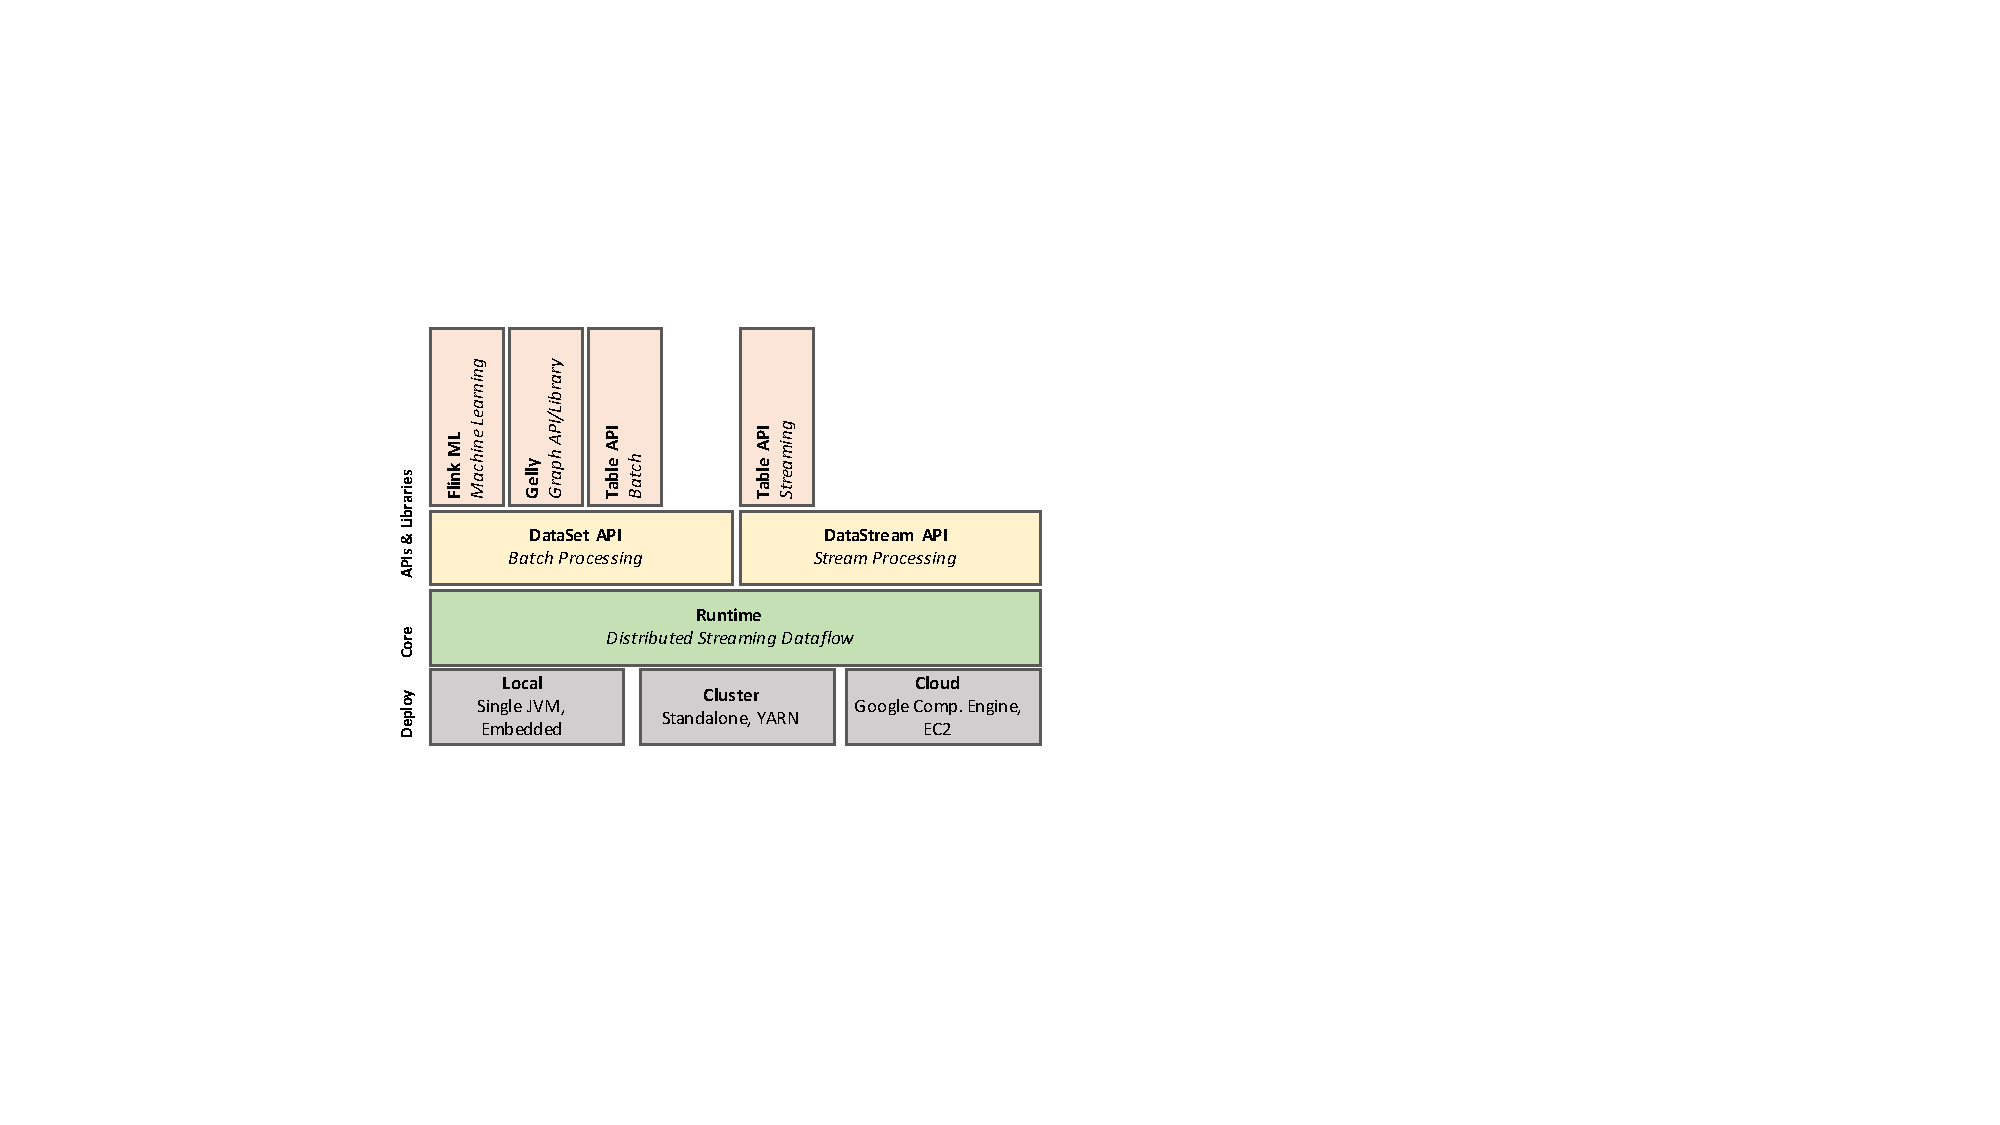
\includegraphics[width=.88\textwidth,natheight=590,natwidth=500]{figs/stack.pdf}
			\vspace{-3mm}
			\caption{The Flink software stack.}
			\vspace{-3mm}
			\label{fig:stack}
          \end{figure}
      \end{minipage}
      % \hspace{0.05\linewidth}
      \begin{minipage}{0.5\linewidth}
          \begin{figure}[H]
				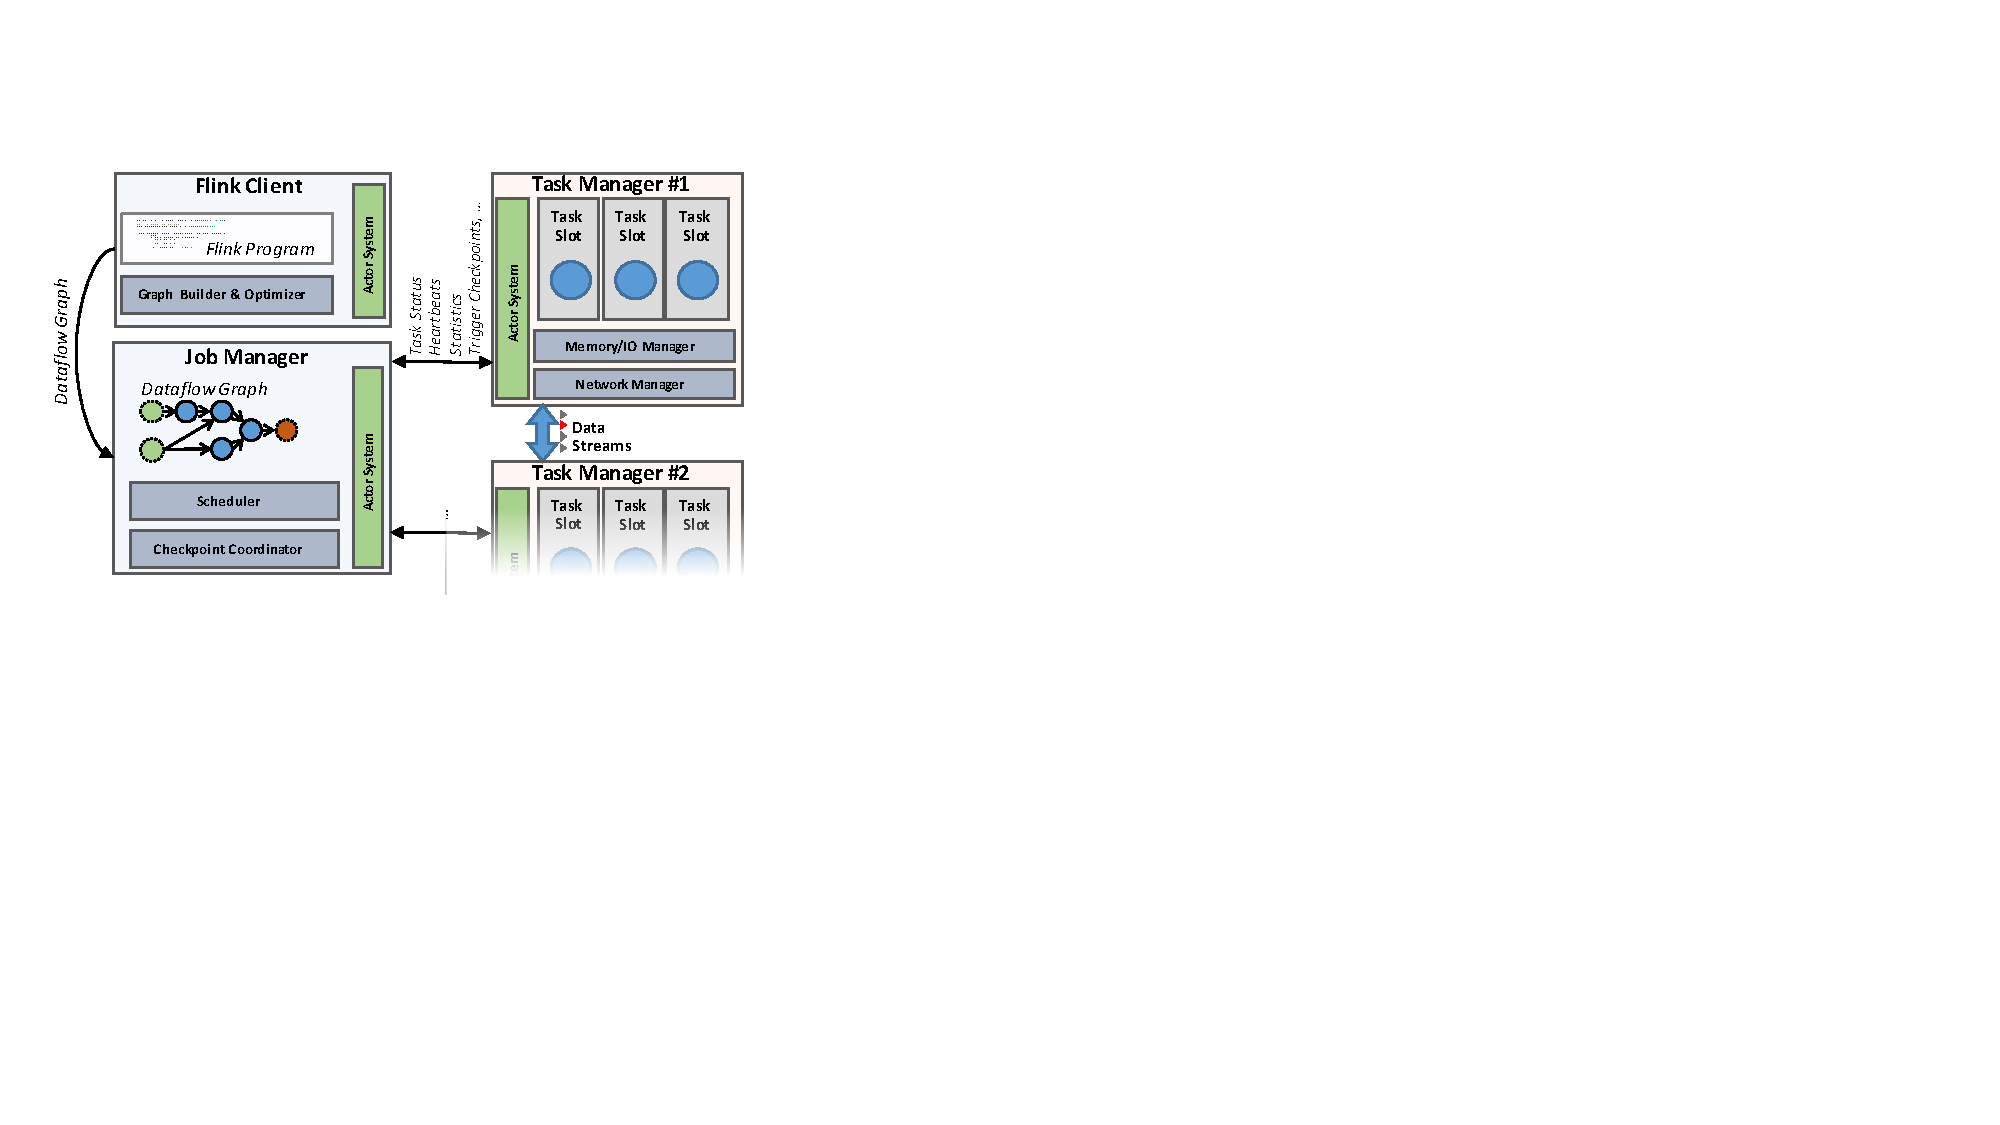
\includegraphics[width=.95\textwidth,natheight=317,natwidth=204]{figs/architecture.pdf}
    			\vspace{-2.5mm}
    			\caption{The Flink process model.}
    			\label{fig:process-model}
          \end{figure}
      \end{minipage}
  \end{minipage}
\end{figure}


% \vspace{-3mm}
\section{The Common Fabric: Streaming Dataflows}
\label{sec:execution}
\vspace{-3mm}

Although users can write Flink programs using a multitude of APIs, all Flink programs eventually compile down to a common representation: the dataflow graph. The dataflow graph is executed by Flink's runtime engine, the common layer underneath both the batch processing (DataSet) and stream processing (DataStream) APIs.

\vspace{-2mm}
\subsection{Dataflow Graphs}
\vspace{-2mm}
The dataflow graph as depicted in \autoref{fig:dataflow} is a directed acyclic graph (DAG) that consists of: (i) stateful operators  and (ii) data streams that represent data produced by an operator and are available for consumption by operators. Since dataflow graphs are executed in a data-parallel fashion, operators are parallelized into one or more parallel instances called \emph{subtasks} and streams are split into one or more \emph{stream partitions} (one partition per producing subtask). 
The stateful operators, which may be stateless as a special case implement all of the processing logic  (e.g., filters, hash joins and stream window functions). Many of these operators are implementations of textbook versions of well known algorithms. In \autoref{sec:streaming}, we provide details on the implementation of windowing operators. Streams distribute data between producing and consuming operators in various patterns, such as point-to-point, broadcast, re-partition, fan-out, and merge.

\begin{figure}[t!]
\begin{minipage}{1.1\linewidth}
      \centering
       \hspace{-0.1\linewidth}
      \begin{minipage}{0.55\linewidth}
        \begin{figure}[H]
        \centering
        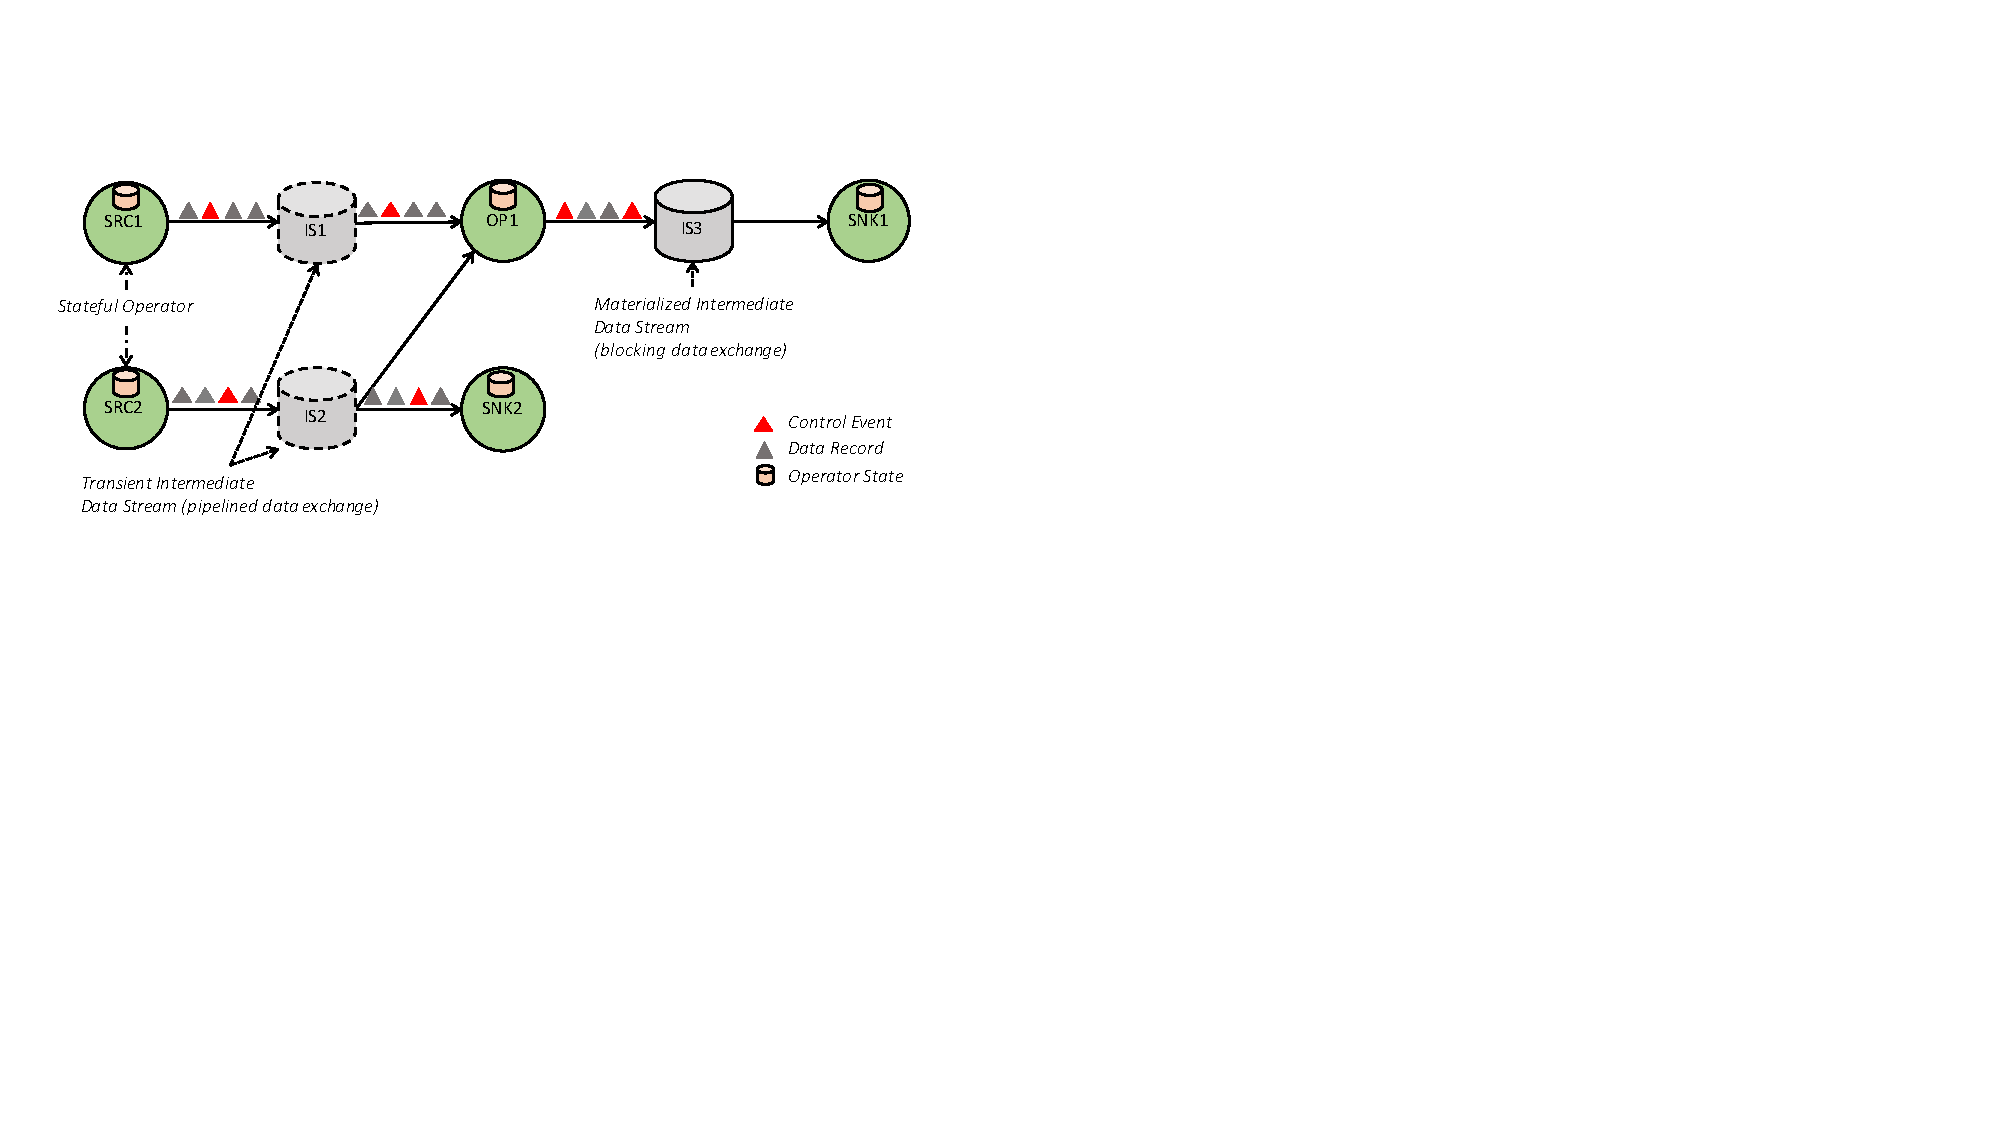
\includegraphics[width=.999\textwidth,natheight=960,natwidth=540]{figs/dataflow.pdf}
        \vspace{-5mm}
        \caption{A simple dataflow graph.}
        \label{fig:dataflow}
        \end{figure}
      \end{minipage}
      \hspace{0.03\linewidth}
      % \vspace{-3mm}
      \begin{minipage}{0.32\linewidth}
          \begin{figure}[H]
				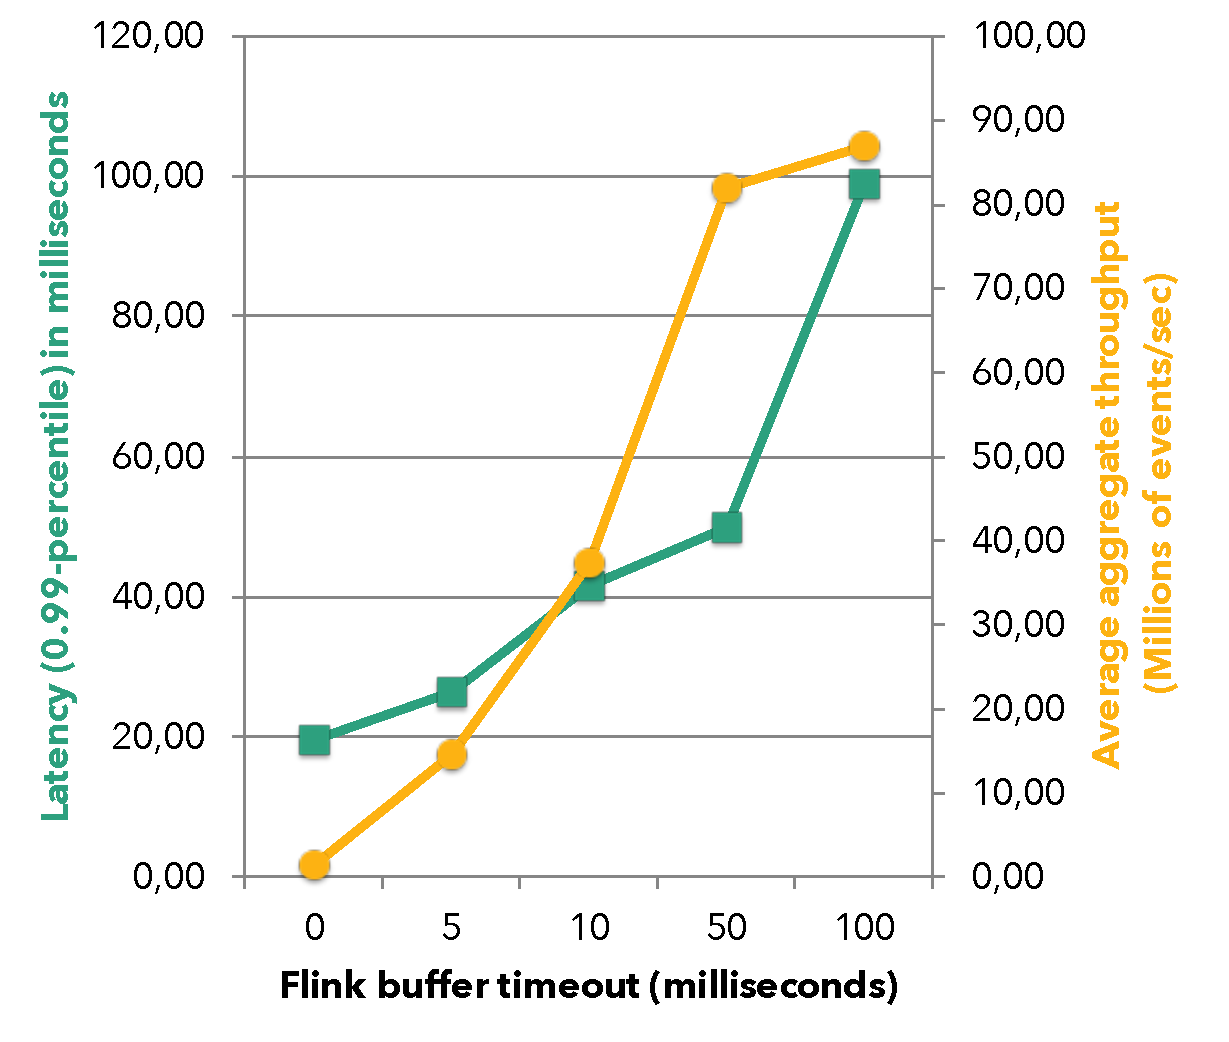
\includegraphics[width=.99\textwidth,natheight=590,natwidth=500]{figs/latency-throughput.pdf}
				\vspace{-7mm}
    			\caption{The effect of buffer-timeout in latency and throughput.}
    			\label{fig:latency-throughput}
          \end{figure}
      \end{minipage}
  \end{minipage}
  \vspace{-4mm}
\end{figure}


\subsection{Data Exchange through Intermediate Data Streams}
Flink's intermediate data streams are the core abstraction for data-exchange between operators. An intermediate data stream represents a logical handle to the data that is produced by an operator and can be consumed by one or more operators. Intermediate streams are logical in the sense that the data they point to may or may not be materialized on disk. The particular behavior of a data stream is parameterized by the higher layers in Flink (e.g., the program optimizer used by the DataSet API). 


\para{Pipelined and Blocking Data Exchange.} \emph{Pipelined intermediate streams} exchange data between concurrently running producers and consumers resulting in pipelined execution. As a result, pipelined streams propagate back pressure from consumers to producers, modulo some elasticity via intermediate buffer pools, in order to compensate for short-term throughput fluctuations. Flink uses pipelined streams for continuous streaming programs, as well as for many parts of batch dataflows, in order to avoid materialization when possible. \emph{Blocking streams} on the other hand are applicable to bounded data streams. A blocking stream buffers all of the producing operator's data before making it available for consumption, thereby separating the producing and consuming operators into different execution stages. Blocking streams naturally require more memory, frequently spill to secondary storage, and do not propagate backpressure. They are used to isolate successive operators against each other (where desired) and in situations where plans with pipeline-breaking operators, such as sort-merge joins may cause distributed deadlocks.

\para{Balancing Latency and Throughput.} Flink's data-exchange mechanisms are implemented around the exchange of buffers. When a data record is ready on the producer side, it is serialized and split into one or more buffers (a buffer can also fit multiple records) that can be forwarded to consumers. A buffer is sent to a consumer either i) as soon as it is full or ii) when a timeout condition is reached. This enables Flink to achieve high throughput by setting the size of buffers to a high value (e.g., a few kilobytes), as well as low latency by setting the buffer timeout to a low value (e.g., a few milliseconds). \autoref{fig:latency-throughput} shows the effect of buffer-timeouts on the throughput and latency of delivering records in a simple streaming grep job on 30 machines (120 cores). Flink can achieve an observable 99$^{\mbox{\small{th}}}$-percentile latency of 20ms. The corresponding throughput is 1.5 million events per second. As we increase the buffer timeout, we see an increase in latency with an increase in throughput, until full throughput is reached (i.e., buffers fill up faster than the timeout expiration). At a buffer timeout of 50ms, the cluster reaches a throughput of more than 80 million events per second with a 99$^{\mbox{\small{th}}}$-percentile latency of 50ms.

\para{Control Events.} Apart from exchanging data, streams in Flink communicate different types of control events. These are special events injected in the data stream by operators, and are delivered in-order along with all other data records and events within a stream partition. The receiving operators react to these events by performing certain actions upon their arrival. Flink uses lots of special types of control events, including: \vspace{-2mm}
\begin{itemize}
\item \textit{checkpoint barriers} that coordinate checkpoints by dividing the stream into pre-checkpoint and post-checkpoint (discussed in \autoref{sec:fault-tolerance}), \vspace{-3mm}
\item \textit{watermarks} signaling the progress of event-time within a stream partition (discussed in \autoref{sec:streaming-time}), \vspace{-3mm}
\item \textit{iteration barriers} signaling that a stream partition has reached the end of a superstep, in Bulk/Stale-Synchronous-Parallel iterative algorithms on top of cyclic dataflows (discussed in \autoref{sec:batch-iterations}). \vspace{-1mm}
\end{itemize}

As mentioned above, control events assume that a stream partition preserves the order of records. To this end, unary operators in Flink that consume a single stream partition, \emph{guarantee a FIFO order of records}. However, operators receiving more than one stream partition merge the streams in arrival order, in order to keep up with the streams' rates and avoid back pressure. As a result, streaming dataflows in Flink do not provide ordering guarantees after any form of repartitioning or broadcasting and the responsibility of dealing with out-of-order records is left to the operator implementation. We found that this arrangement gives the most efficient design, as most operators do not require deterministic order (e.g., hash-joins, maps), and operators that need to compensate for out-of-order arrivals, such as event-time windows can do that more efficiently as part of the operator logic.

\vspace{-3mm}
\subsection{Fault Tolerance}
\label{sec:fault-tolerance}
\vspace{-2mm}
Flink offers reliable execution with strict exactly-once-processing consistency guarantees and deals with failures via checkpointing and partial re-execution. The general assumption the system makes to effectively provide these guarantees is that the data sources are persistent and replayable. Examples of such sources are files and durable message queues (e.g., Apache Kafka). In practice, non-persistent sources can also be incorporated by keeping a write-ahead log within the state of the source operators.

The checkpointing mechanism of Apache Flink builds on the notion of distributed consistent snapshots to achieve exactly-once-processing guarantees. The possibly unbounded nature of a data stream makes re-computation upon recovery impractical, as possibly months of computation will need to be replayed for a long-running job. To bound recovery time, Flink takes a snapshot of the state of operators, including the current position of the input streams at regular intervals.

The core challenge lies in taking a consistent snapshot of all parallel operators without halting the execution of the topology. In essence, the snapshot of all operators should refer to the same logical time in the computation. The mechanism used in Flink is called Asynchronous Barrier Snapshotting (ABS~\cite{carbone2015lightweight}). Barriers are control records injected into the input streams that correspond to a logical time and logically separate the stream to the part whose effects will be included in the current snapshot and the part that will be snapshotted later.

\begin{figure}[t!]
	\centering
  	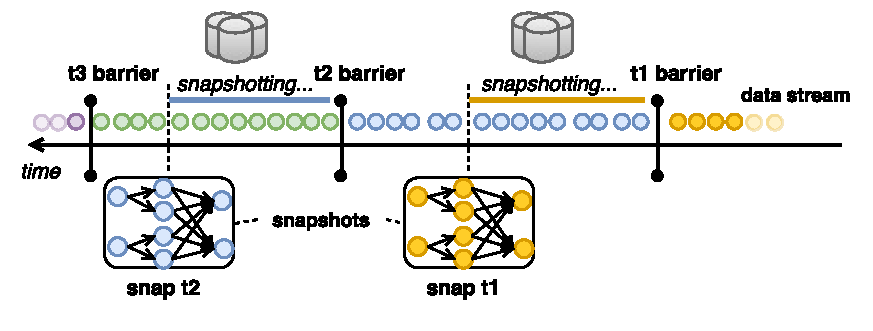
\includegraphics[width=.75\textwidth,natheight=419,natwidth=159]{figs/snaps.pdf}
  	\vspace{-6mm}
	\caption{Asynchronous Barrier Snapshotting.}
	\vspace{-2mm}
	\label{fig:snapshots}
\end{figure}

An operator receives barriers from upstream and first performs an alignment phase, making sure that the barriers from all inputs have been received. Then, the operator writes its state (e.g., contents of a sliding window, or custom data structures) to durable storage (e.g., the storage backend can be an external system such as HDFS). Once the state has been backed up, the operator forwards the barrier downstream. Eventually, all operators will register a snapshot of their state and a global snapshot will be complete. For example, in \autoref{fig:snapshots} we show that \emph{snapshot t2} contains all operator states that are the result of consuming all records before \emph{t2 barrier}. ABS bears resemblances to the Chandy-Lamport algorithm for asynchronous distributed snapshots \cite{chandy1985distributed}. However, because of the DAG structure of a Flink program, ABS does not need to checkpoint in-flight records, but solely relies on the aligning phase to apply all their effects to the operator states. This guarantees that the data that needs to be written to reliable storage is kept to the theoretical minimum (i.e., only the current state of the operators).

Recovery from failures reverts all operator states to their respective states taken from the last successful snapshot and restarts the input streams starting from the latest barrier for which there is a snapshot. The maximum amount of re-computation needed upon recovery is limited to the amount of input records between two consecutive barriers. Furthermore, partial recovery of a failed subtask is possible by additionally replaying unprocessed records  buffered at the immediate upstream subtasks \cite{carbone2015lightweight}.

\vspace{1mm}
\noindent ABS provides several benefits:
\begin{inparaenum}[i)]
\item it guarantees exactly-once state updates without ever pausing the computation
\item it is completely decoupled from other forms of control messages, (e.g., by events that trigger the computation of windows and thereby do not restrict the windowing mechanism to multiples of the checkpoint interval) and
\item it is completely decoupled from the mechanism used for reliable storage, allowing state to be backed up to file systems, databases, etc., depending on the larger environment in which Flink is used.
\end{inparaenum}

\vspace{-3mm}
\subsection{Iterative Dataflows}
\label{sec:iterations}
\vspace{-2mm}
Incremental processing and iterations are crucial for applications, such as graph processing and machine learning. Support for iterations in data-parallel processing platforms typically relies on submitting a new job for each iteration or by adding additional nodes to a running DAG \cite{DBLP:journals/pvldb/BuHBE10, DBLP:conf/hotcloud/ZahariaCFSS10} or feedback edges \cite{murray2013naiad}. Iterations in Flink are implemented as  \emph{iteration steps}, special operators that themselves can contain an execution graph (\autoref{fig:iterations}). To maintain the DAG-based runtime and scheduler, Flink allows for iteration ``head'' and ``tail'' tasks that are \emph{implicitly} connected with feedback edges. The role of these tasks is to establish an active feedback channel to the iteration step and provide coordination for processing data records in transit within this feedback channel. Coordination is needed for implementing any type of structured parallel iteration model, such as the Bulk Synchronous Parallel (BSP) model and is implemented using control event. We explain how iterations are implemented in the DataStream and DataSet APIs in \autoref{sec:stream-iterations} and  \autoref{sec:batch-iterations}, respectively. 


% \vspace{-4mm}
\section{Stream Analytics on Top of Dataflows}
\label{sec:streaming}
\vspace{-3mm}

Flink's DataStream API implements a full stream-analytics framework on top of Flink's runtime, including the mechanisms to manage time such as out-of-order event processing, defining windows, and maintaining and updating user-defined state. The streaming API is based on the notion of a DataStream, a (possibly unbounded) immutable collection of elements of a given type. Since Flink's runtime already supports pipelined data transfers, continuous stateful operators, and a fault-tolerance mechanism for consistent state updates, overlaying a stream processor on top of it essentially boils down to implementing a windowing system and a state interface. As noted, these are invisible to the runtime, which sees windows as just an implementation of stateful operators. 

\vspace{-3mm}
\subsection{The Notion of Time}
\label{sec:streaming-time}
\vspace{-2mm}
Flink distinguishes between two notions of time: i) event-time, which denotes the time when an event originates (e.g., the timestamp associated with a  signal arising from a sensor, such as a mobile device) and ii) processing-time, which is the wall-clock time of the machine that is processing the data.

In distributed systems there is an arbitrary skew between event-time and processing-time \cite{akidau2015dataflow}. This skew may mean arbitrary delays for getting an answer based on event-time semantics. To avoid arbitrary delays, these systems regularly insert special events called \emph{low watermarks} that mark a global progress measure. In the case of time progress for example, a watermark includes a time attribute $t$ indicating that all events lower than $t$ have already entered an operator. The watermarks aid the execution engine in processing events in the correct event order and serialize operations, such as window computations via a unified measure of progress.

Watermarks originate at the sources of a topology, where we can determine the time inherent in future elements. The watermarks propagate from the sources throughout the other operators of the data flow. Operators decide how they react to watermarks. Simple operations, such as map or filter just forward the watermarks they receive, while more complex operators that do calculations based on watermarks (e.g., event-time windows) first compute results triggered by a watermark and then forward it. If an operation has more than one input, the system only forwards the minimum of the incoming watermarks to the operator thereby ensuring correct results.

Flink programs that are based on processing-time rely on local machine clocks, and hence possess a less reliable notion of time, which can lead to inconsistent replays upon recovery. However, they exhibit lower latency. Programs that are based on event-time provide the most reliable semantics, but may exhibit latency due to event-time-processing-time lag. Flink includes a third notion of time as a special case of event-time called \emph{ingestion-time}, which is the time that events enter Flink. That achieves a lower processing latency than event-time and leads to more accurate results in comparison to processing-time.


\begin{figure}[t!]
  \centering
    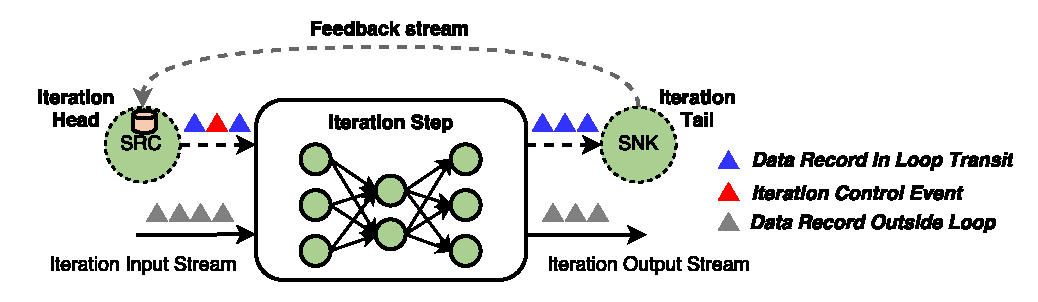
\includegraphics[width=.75\textwidth,natwidth=498,natheight=145]{figs/iterations.pdf}
    \vspace{-6mm}
  \caption{The iteration model of Apache Flink.}
  \vspace{-2mm}
  \label{fig:iterations}
\end{figure}

\vspace{-3mm}
\subsection{Stateful Stream Processing}
\vspace{-2mm}
While most operators in Flink's DataStream API look like functional, side-effect-free operators, they provide support for efficient stateful computations. State is critical to many applications, such as machine-learning model building, graph analysis, user session handling, and window aggregations. There is a plethora of different types of states depending on the use case. For example, the state can be something as simple as a counter or a sum or more complex, such as a classification tree or a large sparse matrix often used in machine-learning applications. Stream windows are  stateful operators that assign records to continuously updated buckets kept in memory as part of the operator state. 

In Flink state is made explicit and is incorporated in the API by providing: i)~operator interfaces or annotations to statically register explicit local variables within the scope of an operator and  ii)~an operator-state abstraction for declaring partitioned key-value states and their associated operations. Users can also configure how the state is stored and checkpointed using the StateBackend abstractions provided by the system, thereby allowing highly flexible custom state management in streaming applications. Flink's checkpointing mechanism (discussed in \autoref{sec:fault-tolerance}) guarantees that any registered state is durable with exactly-once update semantics. 
\vspace{-8mm}

% As a simple example consider a map operator that computes a continuous average for a given stocks price. For this we need to keep a state with the current count and total sum for each stock in order to compute the average:

% \begin{lstlisting}[language=Java]
% val priceStream: DataStream[(String,Double)] = ...
 
% val avgPerStock : DataStream[(String, Double)] = source.keyBy(0).mapWithState(
%     (in, state: Option[(Int, Double)]) => {
% 		val (count, sum) = state.getOrElse((0,0.0))
% 		val newState = (count + 1, sum + in._2)
% 		((in._1, newState._2/newState._1), newState)
% 	}
% \end{lstlisting}

\subsection{Stream Windows}
\vspace{-2mm}
Incremental computations over unbounded streams are often evaluated over continuously evolving logical views, called windows. Apache Flink incorporates windowing within a stateful operator that is configured via a flexible declaration composed out of three core functions: a window \textit{assigner} and optionally a \textit{trigger} and an \textit{evictor}. All three functions can be selected among a pool of common predefined implementations (e.g., sliding time windows) or can be explicitly defined by the user (i.e., user-defined functions).

More specifically, the assigner is responsible for assigning each record to logical windows. For example, this decision can be based on the timestamp of a record when it comes to event-time windows. Note that in the case of sliding windows, an element can belong to multiple logical windows. An optional trigger defines when the operation associated with the window definition is performed. Finally, an optional evictor determines which records to retain within each window. Flink's window assignment process is uniquely capable of covering all known window types such as periodic time- and count-windows, punctuation, landmark, session and delta windows. Note that Flink's windowing capabilities incorporate out-of-order processing seamlessly, similarly to Google Cloud Dataflow \cite{akidau2015dataflow} and, in principle, subsume these windowing models. For example, below is a window definition with a range of 6 seconds that slides every 2 seconds (the assigner). The window results are computed once the watermark passes the end of the window (the trigger).

\begin{lstlisting}[language=Java]
stream
  .window(SlidingTimeWindows.of(Time.of(6, SECONDS), Time.of(2, SECONDS))
  .trigger(EventTimeTrigger.create())
\end{lstlisting}

\noindent A global window creates a single logical group. The following example defines a global window (i.e., the assigner) that invokes the operation on every 1000 events (i.e., the trigger) while keeping the last 100 elements (i.e., the evictor). 

\begin{lstlisting}[language=Java]
stream
  .window(GlobalWindow.create())
  .trigger(Count.of(1000))
  .evict(Count.of(100))
\end{lstlisting}

Note that if the stream above is partitioned on a key before  windowing, the window operation above is \textit{local} and thus does not require coordination between workers. This mechanism can be used to implement a wide variety of windowing functionality \cite{akidau2015dataflow}. 

\vspace{-3mm}
\subsection{Asynchronous Stream Iterations}
\label{sec:stream-iterations}
\vspace{-2mm}
Loops in streams are essential for several applications, such as incrementally building and training machine learning models, reinforcement learning and graph approximations \cite{feigenbaum2005graph,chandramouli2009fly}.
In most such cases, feedback loops need no coordination. Asynchronous iterations cover the communication needs for streaming applications and differ from parallel optimisation problems that are based on structured iterations on finite data. As presented in \autoref{sec:iterations} and \autoref{fig:iterations}, the execution model of Apache Flink already covers asynchronous iterations, when no iteration control mechanism is enabled. In addition, to comply with fault-tolerance guarantees, feedback streams are treated as operator state within the implicit-iteration head operator and are part of a global snapshot \cite{carbone2015lightweight}. The DataStream API allows for an explicit definition of feedback streams and can trivially subsume support for structured loops over streams \cite{murray2013naiad} as well as progress tracking \cite{chandramouli2009fly}.


%!TEX root = paper.tex

% \vspace{-4mm}
\section{Batch Analytics on Top of Dataflows}
\label{sec:batch}
\vspace{-3mm}
A bounded data set is a special case of an unbounded data stream. Thus, a streaming program that inserts all of its input data in a window can form a “batch” program and “batch processing” should be fully covered by Flink's features that were presented above. However, i) the syntax (i.e., the API for batch computation) can be simplified (e.g., there is no need for artificial global window definitions) and ii) programs that process bounded data sets are amenable to additional optimizations, more efficient book-keeping for fault-tolerance, and staged scheduling.

\vspace{2mm}
\noindent Flink approaches batch processing as follows:\vspace{-3mm}
\begin{itemize}
	\item Batch computations are executed by the same runtime as streaming computations. The runtime executable may be parameterized with blocked data streams to break up large computations into isolated stages that are scheduled successively. \vspace{-3mm}
	\item Periodic snapshotting is turned off when its overhead is high. Instead, fault recovery can be achieved by replaying the lost stream partitions from the latest materialized intermediate stream (possibly the source).\vspace{-3mm}
	\item Blocking operators (e.g., sorts) are simply operator implementations that happen to block until they have consumed their entire input. The runtime is not aware of whether an operator is blocking or not. These operators use managed memory provided by Flink (either on or off the JVM heap) and can spill to disk if their inputs exceed their memory bounds.\vspace{-3mm}
	\item A dedicated DataSet API provides familiar abstractions for batch computations, namely a bounded fault-tolerant DataSet data structure and transformations on DataSets (e.g., joins, aggregations, iterations).\vspace{-3mm}
	\item A query optimization layer transforms a DataSet program into an efficient executable.\vspace{-3mm}
\end{itemize}

\noindent Below we describe these aspects in greater detail.

\vspace{-3mm}
\subsection{Query Optimization} 
\vspace{-2mm}
Flink's optimizer builds on techniques from parallel database systems such as plan equivalence, cost modeling and interesting-property propagation. However, the arbitrary UDF-heavy DAGs that make up Flink's dataflow programs do not allow a traditional optimizer to employ database techniques out of the box \cite{blackBoxes}, since the operators hide their semantics from the optimizer. For the same reason, cardinality and cost-estimation methods are equally difficult to employ. Flink's runtime supports various execution strategies including repartition and broadcast data transfer, as well as sort-based grouping and sort- and hash-based join implementations. Flink's optimizer enumerates different physical plans based on the concept of interesting properties propagation \cite{scopeOptimizer}, using a cost-based approach to choose among multiple physical plans. The cost includes network and disk I/O as well as CPU cost. To overcome the cardinality estimation issues in the presence of UDFs, Flink's optimizer can use hints that are provided by the programmer.

\vspace{-3mm}
\subsection{Memory Management} 
\vspace{-2mm}
Building on database technology, Flink serializes data into memory segments, instead of allocating objects in the JVM’s heap to represent buffered in-flight data records. Operations such as sorting and joining operate as much as possible on the binary data directly, keeping the serialization and deserialization overhead at a minimum and partially spilling data to disk when needed. To handle arbitrary objects, Flink uses type inference and  custom serialization mechanisms.  By keeping the data processing on binary representation and off-heap, Flink manages to reduce the garbage collection overhead, and use cache-efficient and robust algorithms that scale gracefully under memory pressure.

\vspace{-3mm}
\subsection{Batch Iterations}
\label{sec:batch-iterations}
\vspace{-2mm}
Iterative graph analytics, parallel gradient descent and optimisation techniques have been implemented in the past on top of Bulk Synchronous Parallel (BSP) and Stale Synchronous Parallel (SSP) models, among others. Flink's execution model allows for any type of structured iteration logic to be implemented on top, by using iteration-control events. For instance, in the case of a BSP execution, iteration-control events mark the beginning and the end of supersteps in an iterative computation. Finally, Flink introduces further novel optimisation techniques such as the concept of \emph{delta} iterations \cite{DBLP:journals/pvldb/EwenTKM12}, which can exploit sparse computational dependencies Delta iterations are already exploited by Gelly, Flink's Graph API.  

%!TEX root = paper.tex
% \vspace{-4mm}
\section{Related work}
\vspace{-2mm}
\label{sec:related}
Today, there is a wealth of engines for distributed batch and stream analytical processing. We categorise the main systems below. 

\para{Batch Processing.} Apache Hadoop is one of the most popular open-source systems for large-scale data analysis that is based on the MapReduce paradigm~\cite{DBLP:journals/cacm/DeanG08}. Dryad~\cite{isard2007dryad} introduced embedded user-defined functions in general DAG-based dataflows and was enriched by SCOPE~\cite{scopeOptimizer}, which a language and an SQL optimizer on top of it. Apache Tez~\cite{saha2015apache} can be seen as an open source implementation of the ideas proposed in Dryad. MPP databases \cite{dewitt1990gamma}, and recent open-source implementations like Apache Drill and Impala \cite{kornacker2015impala}, restrict their API to SQL variants. Similar to Flink, Apache Spark \cite{DBLP:conf/hotcloud/ZahariaCFSS10} is a data-processing framework that implements a DAG-based execution engine, provides an SQL optimizer, performs driver-based iterations, and treats unbounded computation as micro-batches. In contrast, Flink is the only system that incorporates
\begin{inparaenum}[i)]
  \item a distributed dataflow runtime that exploits pipelined streaming execution for batch and stream workloads,
  \item exactly-once state consistency through lightweight checkpointing,
  \item native iterative processing,
  \item sophisticated window semantics, supporting out-of-order processing.
\end{inparaenum}

\para{Stream Processing.} There is a wealth of prior work on academic and commercial stream processing systems, such as SEEP, Naiad, Microsoft StreamInsight, and IBM Streams. Many of these systems are based on research in the database community \cite{chandrasekaran2003psoup,abadi2005design,arasu2004stream,chandramouli2014trill,gedik2008spade,migliavacca2010seep,murray2013naiad}. Most of the above systems are either
\begin{inparaenum}[i)]
  \item academic prototypes,
  \item closed-source commercial products, or 
  \item do not scale the computation horizontally on clusters of commodity servers.
\end{inparaenum}
More recent approaches in data streaming enable horizontal scalability and compositional dataflow operators with weaker state consistency guarantees (e.g., at-least-once processing in Apache Storm and Samza). Notably, concepts such as ``out of order processing'' (OOP)~\cite{li2008out} gained significant attraction and were adopted by  MillWheel~\cite{akidau2013millwheel}, Google's internal version of the later offered commercial executor of Apache Beam/Google Dataflow~\cite{akidau2015dataflow}. Millwheel served as a proof of concept for exactly-once low latency stream processing and OOP, thus, being very influential to the evolution of Flink. To the best of our knowledge, Flink is the only open-source project that:
\begin{inparaenum}[i)]
  \item supports event time and out-of-order event processing
  \item provides consistent managed state with exactly-once guarantees
  \item achieves high throughput and low latency, serving both batch and streaming
\end{inparaenum}

\vspace{-4mm}
\section{Acknowledgements}
\vspace{-2mm}
\label{sec:acknowledgements}
The development of the Apache Flink project is overseen by a self-selected team of active contributors to the project. A Project Management Committee (PMC) guides the project's ongoing operations, including community development and product releases. At the current time of writing this, the list of Flink committers are : M\'arton Balassi, Paris Carbone, Ufuk Celebi, Stephan Ewen, Gyula F\'ora, Alan Gates, Greg Hogan, Fabian Hueske, Vasia Kalavri, Aljoscha Krettek, ChengXiang Li, Andra Lungu, Robert Metzger, Maximilian Michels, Chiwan Park, Till Rohrmann, Henry Saputra, Matthias J. Sax, Sebastian Schelter, Kostas Tzoumas, Timo Walther and Daniel Warneke. In addition to these individuals, we want to acknowledge the broader Flink community of more than 180 contributors.

\vspace{-5mm}
\section{Conclusion}
\vspace{-2mm}
\label{sec:conclusions}
In this paper, we presented Apache Flink, a platform that implements a universal dataflow engine designed to perform both stream and batch analytics. Flink's dataflow engine treats operator state and logical intermediate results as first-class citizens and is used by both the batch and a data stream APIs with different parameters. The streaming API that is built on top of  Flink's streaming dataflow engine provides the means to keep recoverable state and to partition, transform, and aggregate data stream windows. While batch computations are, in theory, a special case of a streaming computations, Flink treats them specially, by optimizing their execution using a query optimizer and by implementing blocking operators that gracefully spill to disk in the absence of memory. 

% \begin{thebibliography}{10}
% \itemsep=1pt
% \begin{small}

\vspace{-3mm}
\begin{thebibliography}{10}
\itemsep=1pt
\begin{small}


\bibitem{abadi2005design}
D.~J. Abadi, Y.~Ahmad, M.~Balazinska, U.~Cetintemel, M.~Cherniack, J.-H. Hwang,
  W.~Lindner, A.~Maskey, A.~Rasin, E.~Ryvkina, et~al.
\newblock The design of the Borealis stream processing engine.
\newblock {\em CIDR}, 2005.

\bibitem{akidau2013millwheel}
T.~Akidau, A.~Balikov, K.~Bekiro{\u{g}}lu, S.~Chernyak, J.~Haberman, R.~Lax,
  S.~McVeety, D.~Mills, P.~Nordstrom, and S.~Whittle.
\newblock Millwheel: fault-tolerant stream processing at Internet scale.
\newblock {\em PVLDB}, 2013.

\bibitem{akidau2015dataflow}
T.~Akidau, R.~Bradshaw, C.~Chambers, S.~Chernyak, R.~J.
  Fern{\'a}ndez-Moctezuma, R.~Lax, S.~McVeety, D.~Mills, F.~Perry, E.~Schmidt,
  et~al.
\newblock The dataflow model: a practical approach to balancing correctness,
  latency, and cost in massive-scale, unbounded, out-of-order data processing.
\newblock {\em PVLDB}, 2015.

\bibitem{stratosphere}
A.~Alexandrov, R.~Bergmann, S.~Ewen, J.-C. Freytag, F.~Hueske, A.~Heise,
  O.~Kao, M.~Leich, U.~Leser, V.~Markl, F.~Naumann, M.~Peters, A.~Rheinlaender,
  M.~J. Sax, S.~Schelter, M.~Hoeger, K.~Tzoumas, and D.~Warneke.
\newblock The stratosphere platform for big data analytics.
\newblock {\em VLDB Journal}, 2014.

\bibitem{arasu2004stream}
A.~Arasu, B.~Babcock, S.~Babu, J.~Cieslewicz, M.~Datar, K.~Ito, R.~Motwani,
  U.~Srivastava, and J.~Widom.
\newblock Stream: The stanford data stream management system.
\newblock {\em Technical Report}, 2004.

\bibitem{DBLP:journals/pvldb/BuHBE10}
Y.~Bu, B.~Howe, M.~Balazinska, and M.~D. Ernst.
\newblock {HaLoop: Efficient Iterative Data Processing on Large Clusters}.
\newblock {\em PVLDB}, 2010.

\bibitem{carbone2015lightweight}
P.~Carbone, G.~F{\'o}ra, S.~Ewen, S.~Haridi, and K.~Tzoumas.
\newblock Lightweight asynchronous snapshots for distributed dataflows.
\newblock {\em arXiv:1506.08603}, 2015.

\bibitem{chandramouli2014trill}
B.~Chandramouli, J.~Goldstein, M.~Barnett, R.~DeLine, D.~Fisher, J.~C. Platt,
  J.~F. Terwilliger, and J.~Wernsing.
\newblock Trill: a high-performance incremental query processor for diverse
  analytics.
\newblock {\em PVLDB}, 2014.

\bibitem{chandramouli2009fly}
B.~Chandramouli, J.~Goldstein, and D.~Maier.
\newblock On-the-fly progress detection in iterative stream queries.
\newblock {\em PVLDB}, 2009.

\bibitem{chandrasekaran2003psoup}
S.~Chandrasekaran and M.~J. Franklin.
\newblock Psoup: a system for streaming queries over streaming data.
\newblock {\em VLDB Journal}, 2003.

\bibitem{chandy1985distributed}
K.~M. Chandy and L.~Lamport.
\newblock Distributed snapshots: determining global states of distributed
  systems.
\newblock {\em ACM TOCS}, 1985.

\bibitem{DBLP:journals/cacm/DeanG08}
J.~Dean~et al.
\newblock {MapReduce: simplified data processing on large clusters}.
\newblock {\em Communications of the {ACM}}, 2008.

\bibitem{dewitt1990gamma}
D.~J. DeWitt, S.~Ghandeharizadeh, D.~Schneider, A.~Bricker, H.-I. Hsiao,
  R.~Rasmussen, et~al.
\newblock The gamma database machine project.
\newblock {\em IEEE TKDE}, 1990.

\bibitem{DBLP:journals/pvldb/EwenTKM12}
S.~Ewen, K.~Tzoumas, M.~Kaufmann, and V.~Markl.
\newblock {Spinning Fast Iterative Data Flows}.
\newblock {\em {PVLDB}}, 2012.

\bibitem{feigenbaum2005graph}
J.~Feigenbaum, S.~Kannan, A.~McGregor, S.~Suri, and J.~Zhang.
\newblock On graph problems in a semi-streaming model.
\newblock {\em Theoretical Computer Science}, 2005.

\bibitem{gedik2008spade}
B.~Gedik, H.~Andrade, K.-L. Wu, P.~S. Yu, and M.~Doo.
\newblock Spade: the system s declarative stream processing engine.
\newblock {\em ACM SIGMOD}, 2008.

\bibitem{blackBoxes}
F.~Hueske, M.~Peters, M.~J. Sax, A.~Rheinl{\"a}nder, R.~Bergmann, A.~Krettek,
  and K.~Tzoumas.
\newblock {Opening the Black Boxes in Data Flow Optimization}.
\newblock {\em PVLDB}, 2012.

\bibitem{isard2007dryad}
M.~Isard, M.~Budiu, Y.~Yu, A.~Birrell, and D.~Fetterly.
\newblock Dryad: distributed data-parallel programs from sequential building
  blocks.
\newblock {\em ACM SIGOPS}, 2007.

\bibitem{kornacker2015impala}
M.~Kornacker, A.~Behm, V.~Bittorf, T.~Bobrovytsky, C.~Ching, A.~Choi,
  J.~Erickson, M.~Grund, D.~Hecht, M.~Jacobs, et~al.
\newblock Impala: A modern, open-source sql engine for hadoop.
\newblock {\em CIDR}, 2015.

\bibitem{li2008out}
J.~Li, K.~Tufte, V.~Shkapenyuk, V.~Papadimos, T.~Johnson, and D.~Maier.
\newblock Out-of-order processing: a new architecture for high-performance
  stream systems.
\newblock {\em PVLDB}, 2008.

\bibitem{marz2015big}
N.~Marz and J.~Warren.
\newblock {\em Big Data: Principles and best practices of scalable realtime data systems}.
\newblock Manning Publications Co., 2015.

\bibitem{migliavacca2010seep}
M.~Migliavacca, D.~Eyers, J.~Bacon, Y.~Papagiannis, B.~Shand, and P.~Pietzuch.
\newblock Seep: scalable and elastic event processing.
\newblock {\em ACM Middleware'10 Posters and Demos Track}, 2010.

\bibitem{murray2013naiad}
D.~G. Murray, F.~McSherry, R.~Isaacs, M.~Isard, P.~Barham, and M.~Abadi.
\newblock Naiad: a timely dataflow system.
\newblock {\em ACM SOSP}, 2013.

\bibitem{saha2015apache}
B.~Saha, H.~Shah, S.~Seth, G.~Vijayaraghavan, A.~Murthy, and C.~Curino.
\newblock Apache tez: A unifying framework for modeling and building data
  processing applications.
\newblock {\em ACM SIGMOD}, 2015.

\bibitem{DBLP:conf/hotcloud/ZahariaCFSS10}
M.~Zaharia, M.~Chowdhury, M.~J. Franklin, S.~Shenker, and I.~Stoica.
\newblock {Spark: Cluster Computing with Working Sets}.
\newblock {\em {USENIX HotCloud}}, 2010.

\bibitem{scopeOptimizer}
J.~Zhou, P.-A. Larson, and R.~Chaiken.
\newblock Incorporating partitioning and parallel plans into the scope
  optimizer.
\newblock {\em IEEE ICDE}, 2010.

\end{small}
\end{thebibliography}



% {
% \small
% \bibliographystyle{abbrv}
% \bibliography{references}
% }
% \printbibliography

\end{document}